\documentclass[12pt]{article}

\usepackage{fullpage}
\usepackage{amsmath,amssymb,amsfonts,amsthm}

\usepackage{ebgaramond}
\usepackage[cmintegrals,cmbraces]{newtxmath}
\usepackage{ebgaramond-maths}

\usepackage{braket}
\DeclareMathOperator{\cas}{cas}
\newcommand{\trans}[1]{\ensuremath{{#1}^\intercal}}

\usepackage{color}

\setlength\parskip{2mm}

\usepackage{graphicx}
\usepackage[hidelinks, colorlinks=true, allcolors=blue]{hyperref}

\usepackage[style=authoryear,backend=bibtex]{biblatex} %backend tells biblatex what you will be using to process the bibliography file
\addbibresource{refs.bib}

\begin{document}
\title{A Survey on Temporal Knowledge Graph Completion: Taxonomy, Progress, and Prospects}
\author{Jiapu Wang et al}
\maketitle


\section{What?}


\section{Why?}


\section{How?}

\begin{figure}[h!]
    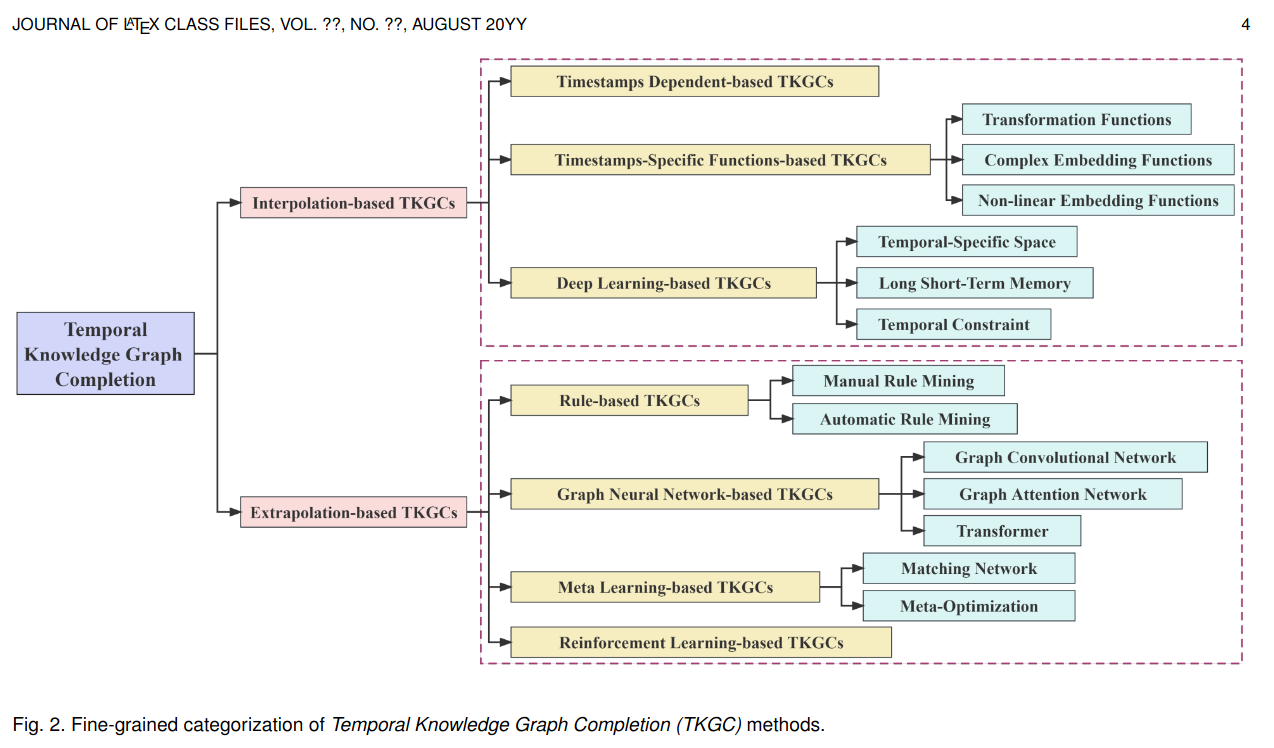
\includegraphics[width=1.1\linewidth]{figures/survey_wang2023_fig01.png}
    \caption{Tổng quan hướng tiếp cận bài toán hoàn thiện đồ thị tri thức động.}
    \label{fig:overview_med_approaches}
\end{figure}

\end{document}